\chapter{Basics}

The chapter is intended to provide a basic understanding of load balancing and kubernetes.
The focus is mainly on the parts that are needed for the further process.
It is not going into detail of everything and won't cover all load balancing features, algorithms and Kubernetes possibilities.
Also, it focuses on features that are commonly used inside the cloud environment, especially Kubernetes and is not covering other scenarios.

\section{Load Balancing}

In simple, a load balancer is a software or hardware device which distributes incoming traffic among a set of servers.
They usually serve as an entrypoint and offer different features in a cloud environment.
\\
The most obvious feature is to distribute traffic to multiple servers.
Load balancers offer a variety of algorithms for how traffic is distributed among endpoints.
The easiest approach is to use ``Random Load Balancing``.
As the name suggests, traffic is distributed randomly to the endpoints.
However, this can result in one endpoint receiving a lot of traffic, and others receiving very little traffic.
To address this issue, the most common algorithm might be ``Round Robin``.
Here traffic is sequentially forwarded to each endpoint.
This method provides an evenly distributed amount of traffic to the endpoint.
There are still scenarios where it might be useful to distribute traffic in another way.
For instance, imagine an endpoint with high resource capacity that is able of processing more load than others.
For this it makes sense to use ``Weight Selection``.
Basically the load balancer is told to send more traffic to the higher weighted endpoints than to others.
Another algorithm is ``Least Request`` where the load balancer tries to determine the endpoint with the least open requests.
This highly depends on the load balancer implementation.
\\
The second feature is to dynamically change the configuration of your load balancer.
In a production environment it is important not to interrupt your services or even dropping connections by restarting some components, especially for critical infrastructure like a load balancer.
This is useful in terms of auto scaling with a dynamic number of endpoints, which may is based upon the current server load.
\\
The third one is to provide a failover for ``High Available`` setups.
This requires some health check mechanism, like TCP or HTTP probes.
These probes are used to determine the endpoints healthiness and mark an endpoint as unhealthy if one or more probes fail.
When an endpoint becomes unhealthy, the load balancer stops forwarding traffic to it.
\\
Load balancers can operate on different levels of the Open Systems Interconnection model (OSI model).
Those are called layer 4 (Transport Layer) or layer 7 (Applikation layer) load balancers.
\\
A layer 4 load balancer takes place on the Transport layer, that means they are handling transport packages like TCP or UDP.
The fact that messages are neither inspected nor decrypted allows them to be forwarded quickly, efficiently, and securely.
\\
A layer 7 load balancer takes place on the Application layer, using protocols such as HTTP and SMTP.
At this level the load balancer does have more information and can perform smarter decisions.
In terms of HTTP this means you can take routing decisions based upon HTTP Headers.
TLS termination is also handled by Layer 7 load balancers.

\section{Kubernetes}

Kubernetes is an open-source container-orchestration platform for automating deployments, scaling and management.

A Cluster contains a so called control-plane which is responsible for the cluster state.
The control-plane is a set of controllers which observe different objects of the cluster, react to changes and trie to bring the cluster into it's desired state.
\\
Each node inside the cluster is running three key components on the host machine: kubelet, kube-proxy and a container runtime.
\\
Kubelet is responsible for the node status, and the containers that are deployed to it.
\\
The container runtime is an application that implements the Container Runtime Interface.
This is used by kubelet to deploy and control containers on the host machine.
\\
Kube-proxy takes care of the networking part.
It is responsible for routing and exposing services.
A more detailed overview can be found in \autoref{sec:kubeproxy}.
\\
\newpage
Kubernetes offers a various set of building blocks ("primitives"), which describe different parts in the cluster to deploy an Application.
Each object shares the same basic data structure.

\begin{itemize}
    \item \textit{apiVersion} \\
    The api version to be used, ether alpha, beta, or stable in different versions.
    \item \textit{kind} \\
    What kind is the object to create.
    \item \textit{metadata} \\
    Name, namespace and other metadata like labels and annotations.
    \item \textit{spec} \\
    The description of the state that is desired.
    The implementation differs for every object.
\end{itemize}

Some objects also have a status field that describes the current state.

\subsection{Pods}
The first basic one is a ``Pod`` that is a group of one or more containers.
The containers share storage, network, and runtime specifications.
\\
Kubernetes manages pods instead of containers directly, so a pod is a wrapper around one or more containers.
\\
There are applications where two containers are tightly coupled together.
Then it can make sense to deploy these containers together in one pod.
This ensures that the containers are deployed on the same node and have the same resources at their disposal, which has a positive effect on performance.
\\
It holds information of the docker image, volumes, ports and more.
A Pod is not created directly, instead it is described inside a Deployment, StatefulSet or DaemonSet.

\subsection{Deployment}

A Deployment takes track of the current state, make changes to an existing Pods in a controlled rate, scaling and more.
It is widely used to deploy applications in a general purpose way.
The ``spec.template`` describes the actual pod created by the deployment, with its metadata and Pod spec.
The \autoref{fig:deployment} illustrates an example deployment, with two containers and ports, inside a pod.
Deployments have a selector which tells the controller which Pod is controlled by this deployment.
The label ``app: foo-bar``is used as the selector and is also set inside the template, so all Pods created by this template are referenced to the deployment.
If applied, Kubernetes will create one pod, according to the replicas field, with two containers.
The containers use the same image, but with different environment variables and Ports.
Those control what the HTTP service of the image will return and on what port it listens.

\begin{figure}[H]
    \centering
    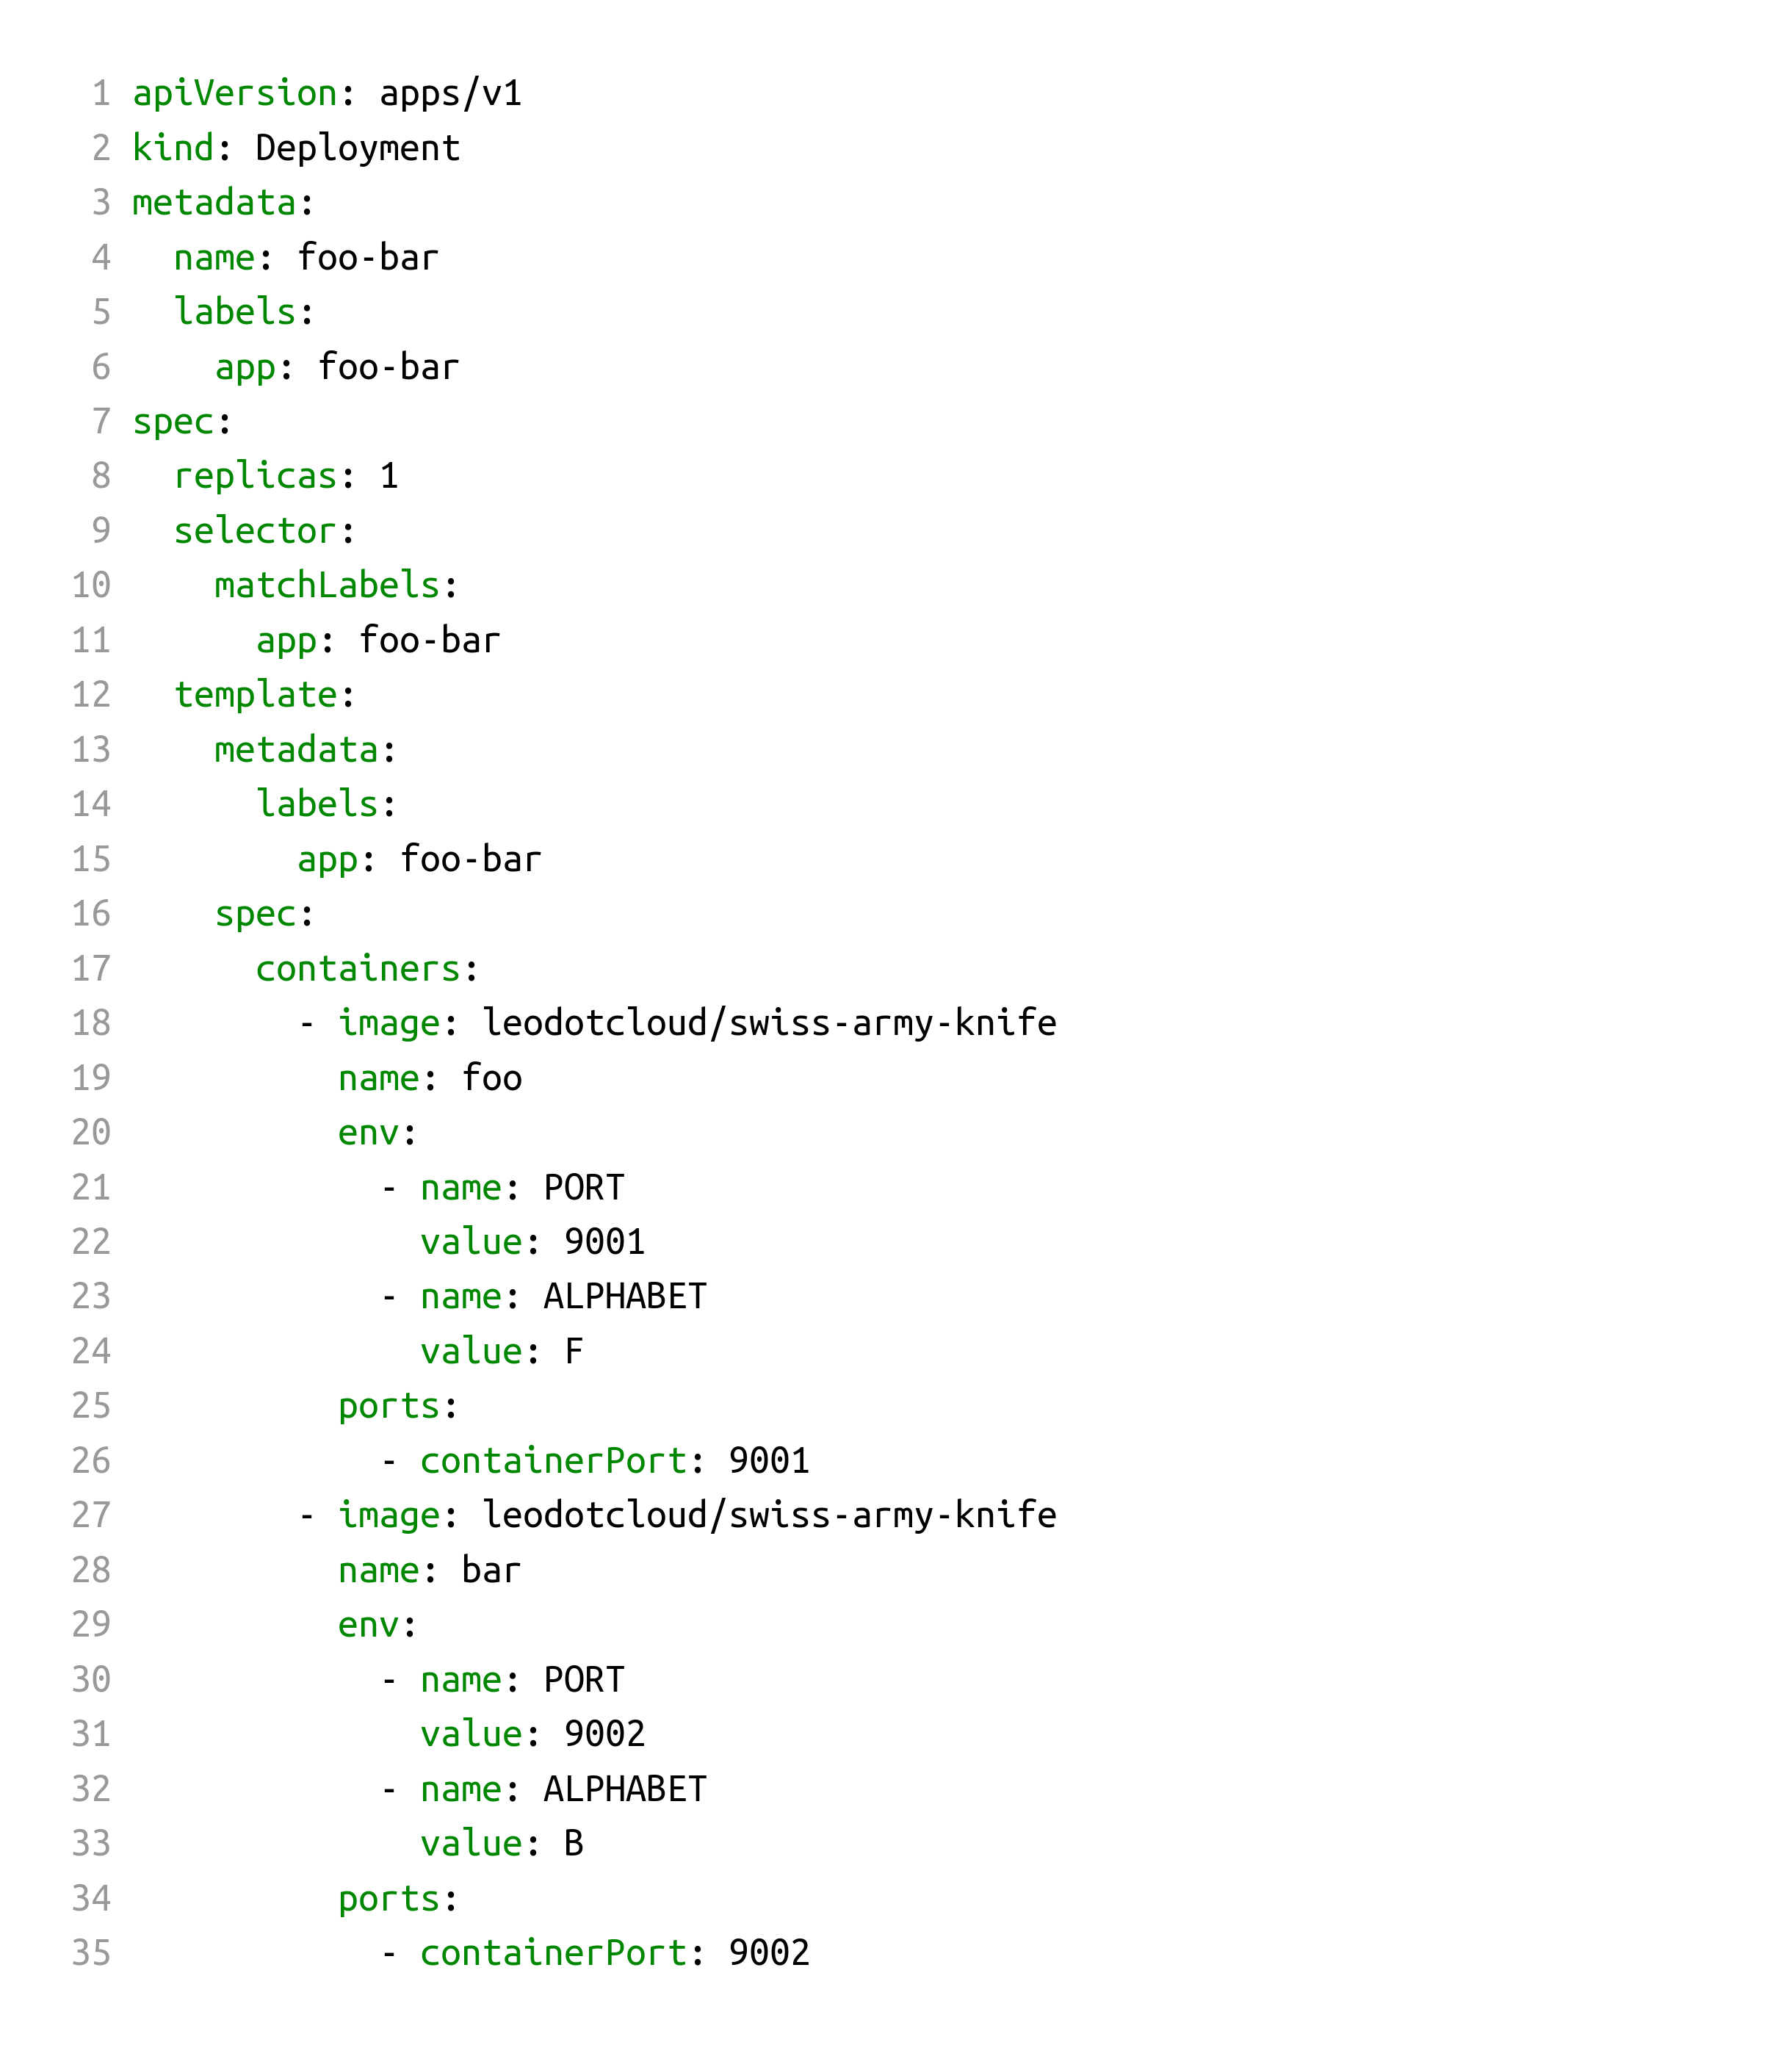
\includegraphics[width=0.7\textwidth, left]{media/02/deployment}
    \caption{Example deployment}
    \label{fig:deployment}
\end{figure}


\subsection{Service}
To expose an application and make it accessible for others, the ``Service`` object is used.
This is an abstraction of the networking layer and decides how to expose an application.
Services are used to open and map one or multiple ports of a Pod.
The actual Pod where the service applies to, is chosen by a selector.
This is important so that the controller knows to which pods the traffic is routed.
To keep track of which endpoints are currently available, the controller automatically creates an endpoint object.

\begin{figure}[H]
    \centering
    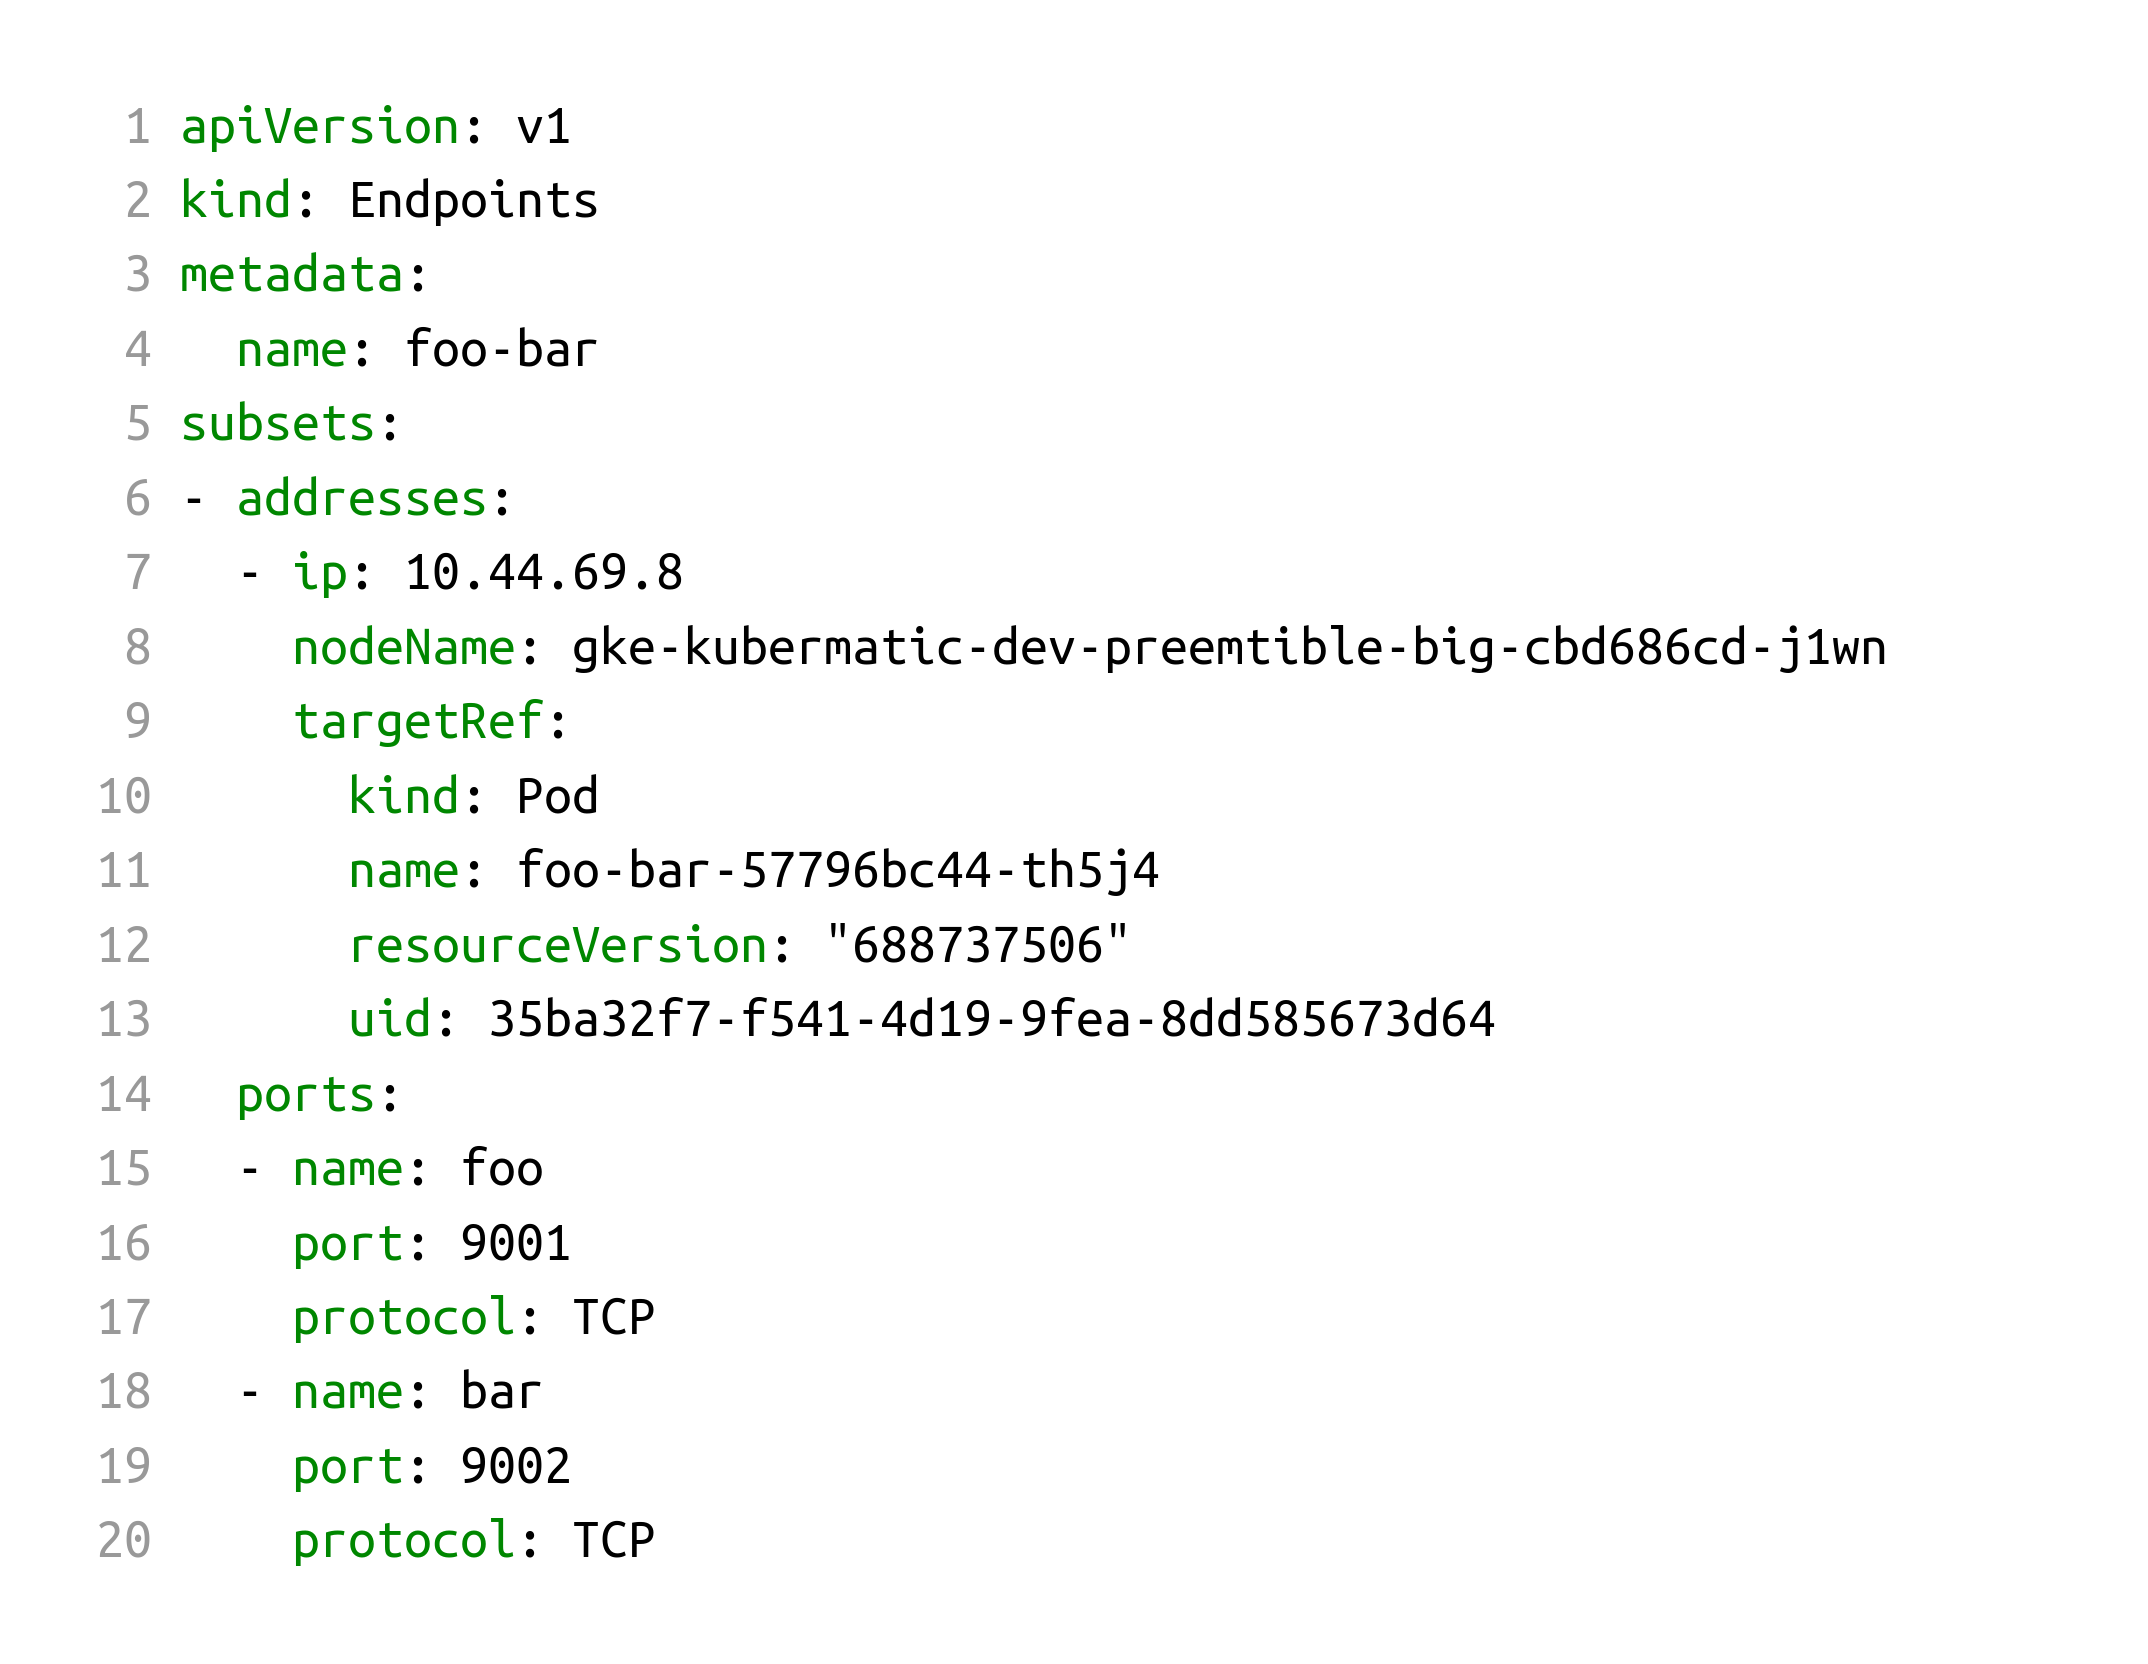
\includegraphics[width=0.7\textwidth, left]{media/02/endpoint}
    \caption{Example endpoints}
    \label{fig:endpoints}
\end{figure}

As \autoref{fig:endpoints} shows, an endpoint holds a list of IP addresses (in this case its just one as only one Pod is deployed), as well as the associated ports.
In addition, the endpoints object is filled with further meta information by the controller.
Kubernetes scans for Pods inside the cluster that match the given selector and updates the corresponding Endpoint object.
For a service without a selector, no associated endpoint is created and must be created otherwise.
TCP, UDP and SCTP are supported as protocols, TCP is the default.

\autoref{fig:service} shows an example service for the previous foo-bar deployment.
It exposes two ports one named foo at Port 8080, and bar at Port 8081.
Target port describes the Port of the actually Pod and could be omitted because it is the same value as port.
The selector is ``app: foo-bar``, which was assigned to the pods as labels in the previous deployment.

\begin{figure}[H]
    \centering
    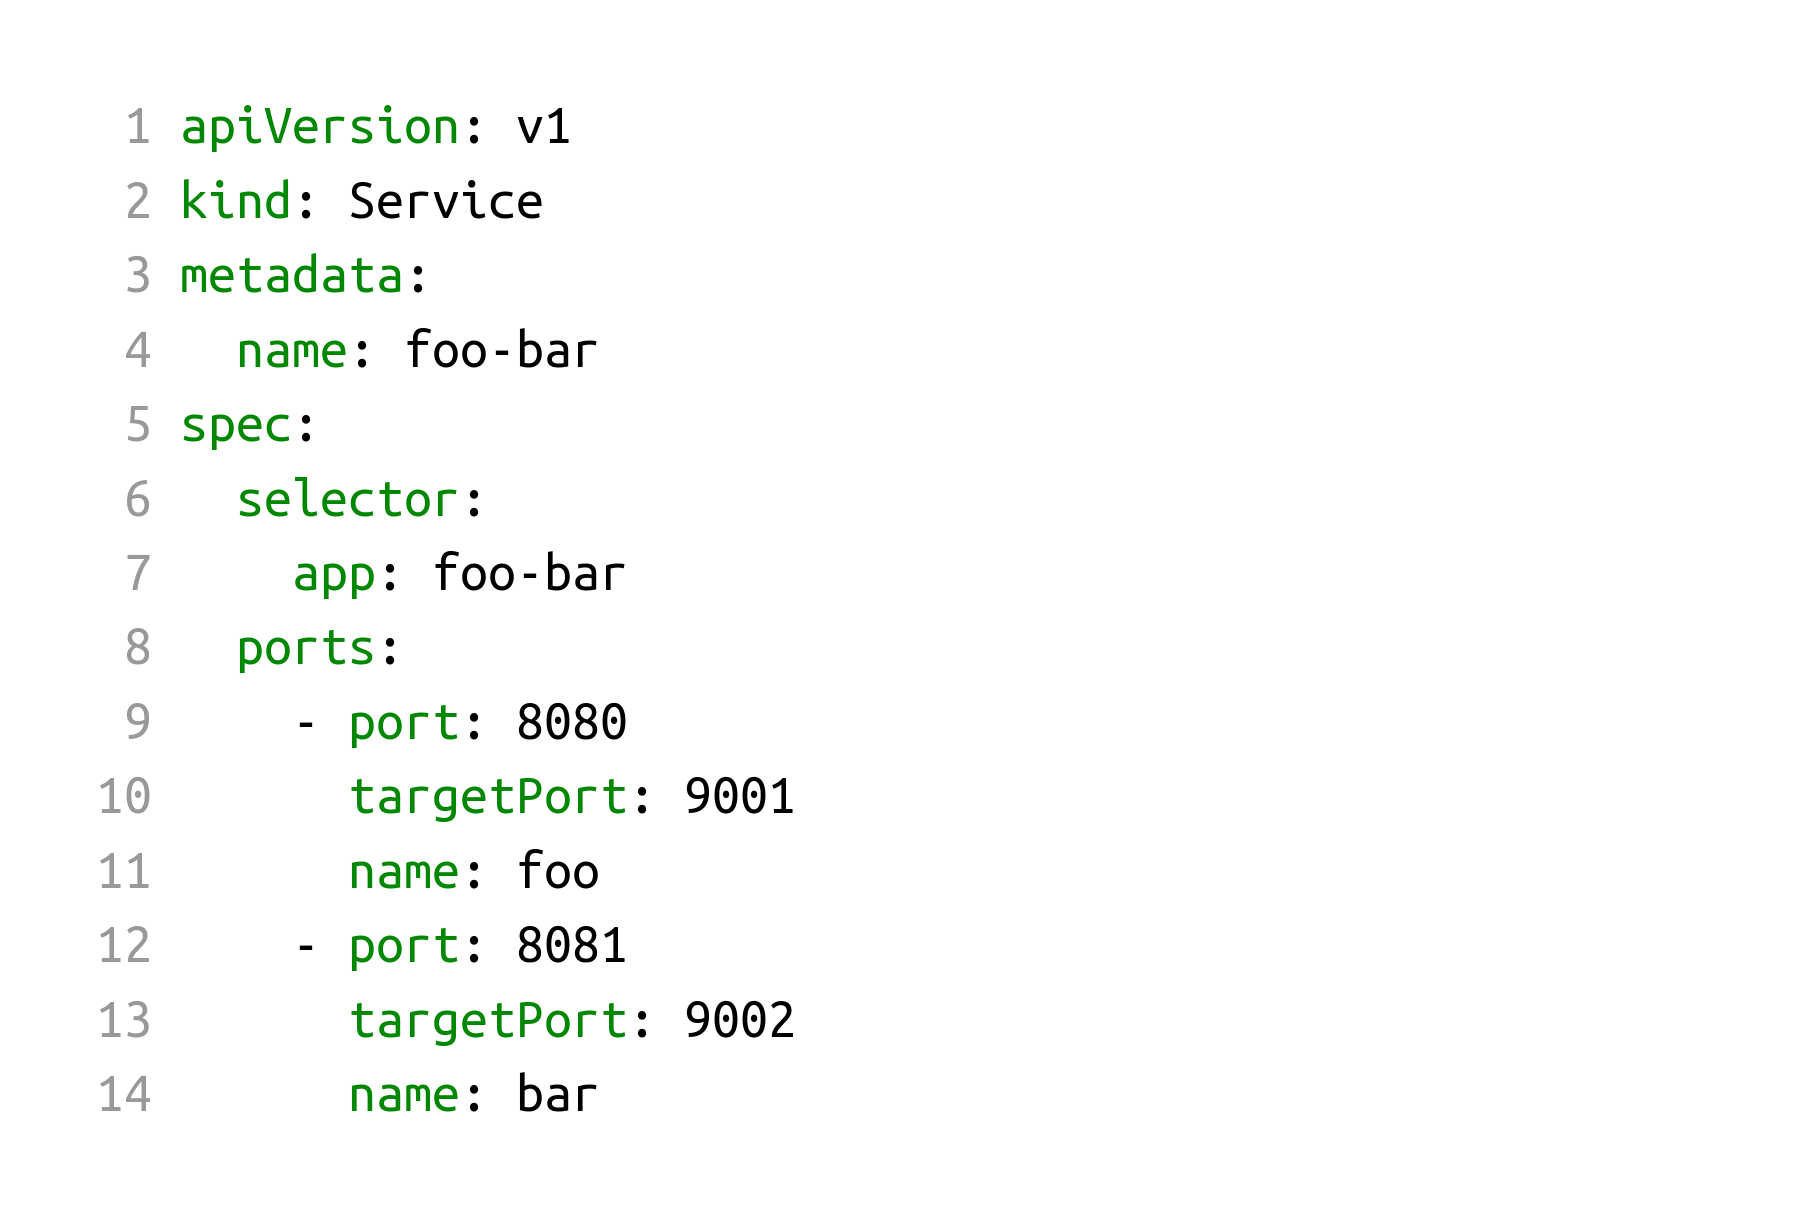
\includegraphics[width=0.7\textwidth, left]{media/02/service}
    \caption{Example service}
    \label{fig:service}
\end{figure}


It offers different types of exposing an application.
Type ClusterIp is the default and exposes the application only to other services inside the cluster.
These services can be addressed via an internal DNS.
Those DNS names follow by default this pattern: my-svc.my-namespace.svc.cluster-domain.example.
This is also the reason why the service name needs to be a valid DNS label.
\\
Type NodePort allocates a random port, by default in between of 30000-32767, and open this on all nodes of the cluster.
Thus, the service is externally accessible on all nodes of the cluster via the allocated port.
\\
Type LoadBalancer does the same as node port with the addition of an external implementation to dynamically create a load balancer and point it to the opened node ports.
This is not implemented by default and requires some extra setup for the cluster, what is explained in more detail in \autoref{sec:ExternalLoadBalancer}.
\\
A service has a corresponding ``Endpoints`` object.
Inside the cluster these are created automatically, via a selector inside the service object, that points to pod.
\subsection{Ingress}

The Ingress Object is built as an addition to services and offers load balancing, TLS Termination or name-based virtual hosting.
Typically, it exposes only HTTP/HTTPS, other applications should make use of the service type NodePort or LoadBalancer.
It provides a number of configurable rules that decide to which backend the traffic is routed.
Thus, applications do not have to be directly exposed via a service, they only need to be internal accessible via ClusterIP.
\autoref{fig:ingress} shows an example of an ingress object that forwards incoming HTTP requests with the /foo path to the foo-service on port 8080, and /bar path to the bar-service on port 8081.

\begin{figure}[H]
    \centering
    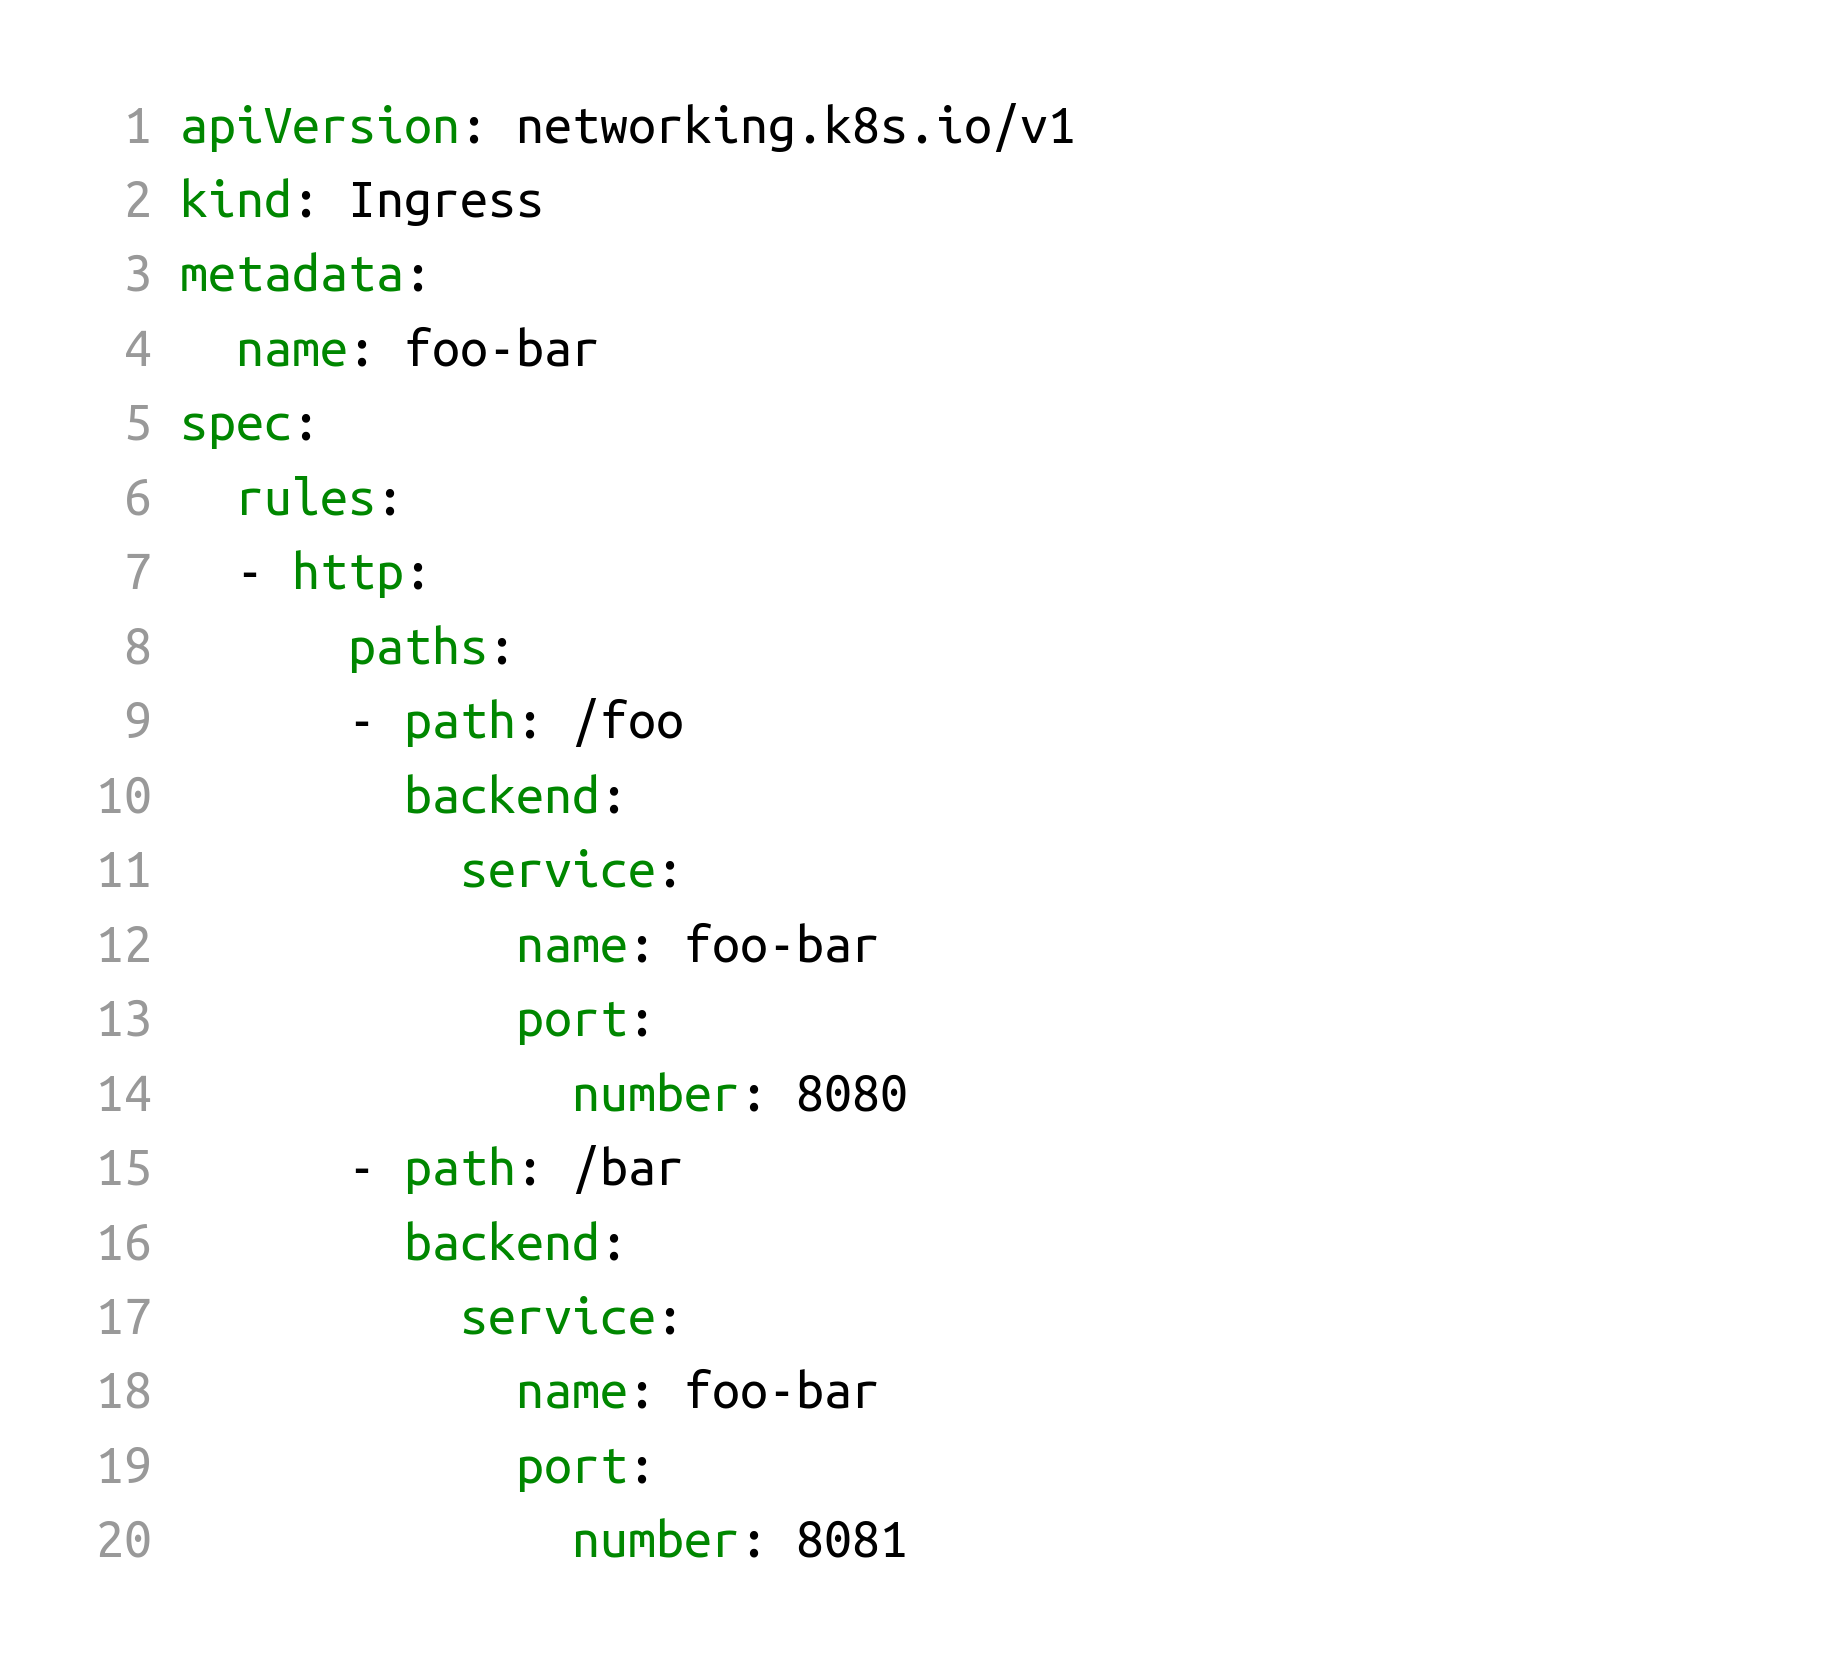
\includegraphics[width=0.7\textwidth, left]{media/02/ingress}
    \caption{Example ingress}
    \label{fig:ingress}
\end{figure}

To fulfill the ingress an IngressController must be installed.
The IngressController and it's purpose will be explained in \autoref{sec:IngressController}.